\win: \menu{\winstart>Программы>KiCAD>KiCAD}

\linux: \verb|user@host$ kicad|

\bigskip
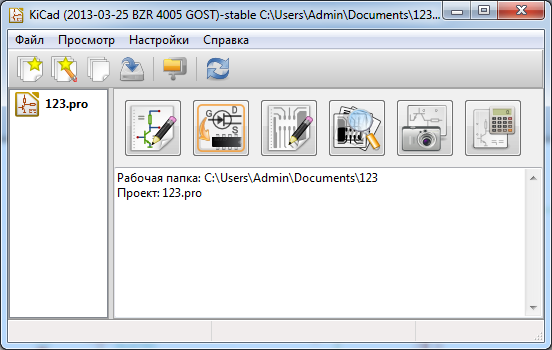
\includegraphics[height=0.8\textheight]{kicad/projman.png}

\bigskip
В верхней части панели \term{менеджера проектов} \prog{kicad} имеются большие
кнопки запуска компонентов KiCad:

\begin{itemize}
\item\icon{kicad/icon_eeschema.png}
\prog{eeschema}\ --- Редактор принципиальных схем
\item\icon{kicad/icon_pcbnew.png}
\prog{pcbnew}\ --- Редактор печатных плат
\item\icon{kicad/icon_cvpcb.png}
\prog{cvpcb}\ --- Программа редактирования \termdef{падстеков}{падстек}
(отверстий и площадок)
\end{itemize}

Каждая кнопка запускает соответствующую программу. Мы будем использовать эти
программы по мере изучения.
